\chapter{Approaches}
\label{ch:approaches_report}


The thesis work follows the ‘User Experience Design cycle’ research methodology, as mentioned in \autoref{ch:background_report} where the theory is established based on own ideas in addition to literature review findings for the first iteration. Then continue to evolve better designs converging towards desired interface by developers. \\ \\

Overall, by analysing the software engineering disciplines as mentioned in \autoref{ch:relatedwork_report}, a theory is established. The prototypes are created based on the established theory and user study mentioned in \autoref{ch:researchmethodology_report} is performed, which follows qualitative and quantitative approaches in assimilating the results. It follows a well established iterative process of UX Design cycle \cite{UX} as seen in the \autoref{fig:ux-design}. \\ \\

Before we start the user study session with any participant in UX Design cycle, we ask the user to read the consent form and sign it. The consent form details what the user study is about, their participation is voluntary, what information we collect, and how we ensure their privacy. It is carefully prepared to be strictly compliant with GDPR data privacy policy. \cite{gdpr} The original copy of consent form is in appendix. \\ \\

Our approach leads an iterative process where initially prototypes with our novel ideas are evaluated by the target users. Next, the evaluation results lead to the requirements gathering phase. Then again, the prototypes are developed based on user feedback and also including any new findings in the literature. The cycle repeats until the desired satisfaction of target users is achieved. \\ \\

In our qualitative research methodology, we concern the feedback of users as an example of emotional feeling on the usability of the designed prototype — for example, such as user behaviour, quotes. On the other hand, in our quantitative research methodology, we analyse some metrics on the results gathered during the evaluation phase — for example, such as time taken to perform the task, performance. \\ \\

For every research question, we formulate the user scenario and what usual Static Code Analysis tool does. Next, what can be done better considering other solution ideas from different Software Engineering domains in addition to our ideas is analysed through the UX Design process. In this process, the metrics mentioned above, which are qualitative and quantitative, are observed. \\

Here is an example of how the implementation approach could get started.

\section{Research Question 1: How to Display the Results of the Same Codebase from Different Analysis Tools}

\textbf{Solution ideas}: \\ \\
1. Display results separately for each tool. \\
2. Combine the results and mark its respective icon in a column to show which tool identifies the particular bug. \\

With above-mentioned possible solution ideas derived after analysing the findings from other software engineering disciplines, i.e., Complex datasets and Issue tracker, two different prototypes are designed using a wireframe tool called Balsamiq \cite{B}. The design lessons adapted from these disciplines are extensibility of columns were integrating the complex datasets into a unified interface. Also, expressiveness concern tackled with issue tracker by having own dashboard instead of overwhelming the user with complete results which are not related to him. Assume the name \textit{toolShort} means a Static Analysis tool capable of giving results in a short time and \textit{toolLong} mean a Static Analysis tool gives results after a long time. \\ \\

\textbf{Prototype 1}: \\ \\

The prototype for solution idea, i.e., separately displaying the results is shown in the following \autoref{fig:toolSeperate}. \\ 

\begin{figure}[hbt!]
	\centering
	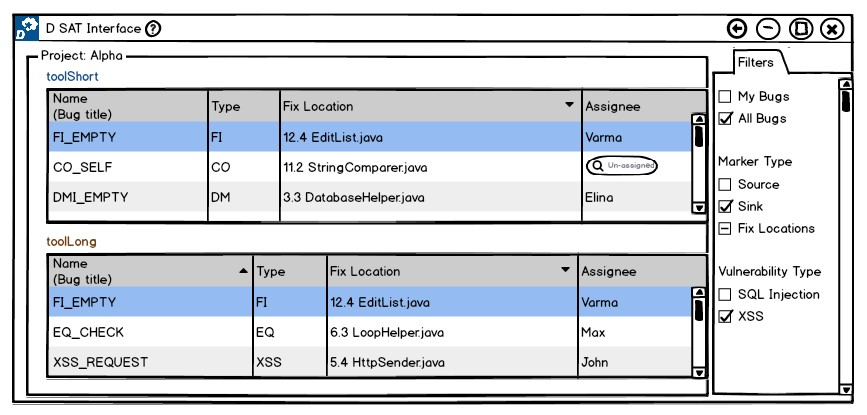
\includegraphics[width=\linewidth]{figures/d_seperate}
	\caption{An interface prototype with tools displaying results separately.}
	\label{fig:toolSeperate}
\end{figure}

\clearpage

\textbf{Prototype 2}: \\ \\

The prototype for solution idea, i.e., combining the results is shown in the following \autoref{fig:toolCombine}. \\ \\

\begin{figure}[hbt!]
	\centering
	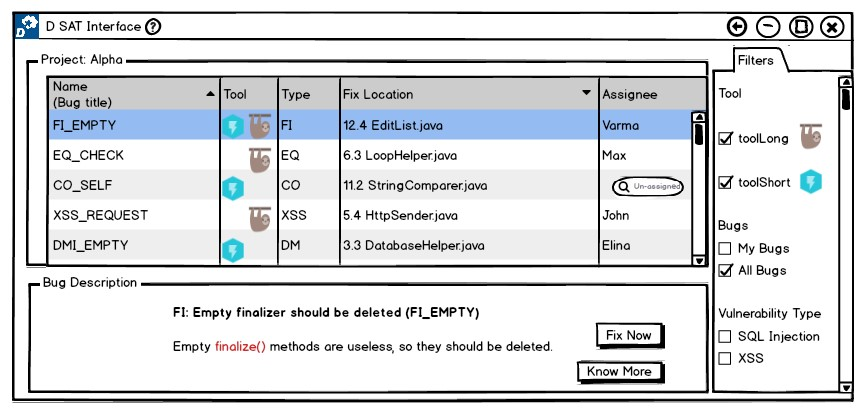
\includegraphics[width=\linewidth]{figures/d_combine}
	\caption{An interface prototype with tools displaying results combined.}
	\label{fig:toolCombine}
\end{figure}

Next, evaluate the designed prototypes as mentioned in chapter \ref{ch:researchmethodology_report}. After evaluation, requirements are gathered based on user feedback and also new findings from the literature, if any. New designs are prototyped as mentioned above and repeats as per User Experience Design cycle. \\ \\

\section{Research Question 2: \\ What Feedback Works to Know that the Bug Fixing is	\\ On-going?}

\textbf{Solution ideas}: \\ \\


1. User selects a bug and tries to fix it with some modifications in code and submit for analysis, and then the bug is shown as pending in status. \\
2. If the modified code fixes the reported bug, then it is shown as ‘fixed’ in status, or else, ‘try again’. \\ \\

With the above mentioned possible solution ideas, we design the prototypes. The prototype \ref{fig:d_pending} illustrates a bug being displayed as ‘pending’ in the status column of bug listing. This scenario happens when a user selects a bug and attempts to fix it then submit for analysis tools. Perhaps the shorter tool, i.e., the tool capable of analysing in less computation time would report back whether the bug got fixed or not. Thereby, the Prototype 2 \ref{fig:d_tryagain} illustrates the bug is not fixed and shown as ‘try again’ in status column as the user attempted to fix earlier. \\ \\

Also, in Prototype 1, it is observed that ‘Fix Now’ button in ‘Bug Description’ window is disabled, which also depicts the tool is analysing the bug in the background. \\

\textbf{Prototype 1}

\begin{figure}[hbt!]
	\centering
	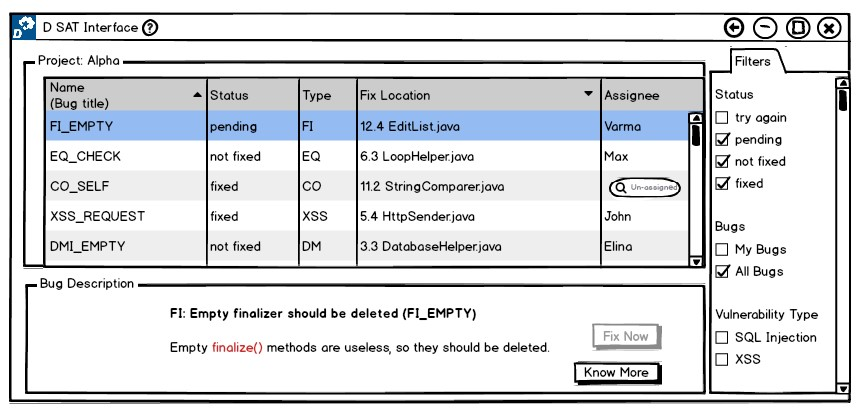
\includegraphics[width=\linewidth]{figures/d_pending}
	\caption{An interface prototype showing pending status.}
	\label{fig:d_pending}
\end{figure}

\textbf{Prototype 2}

\begin{figure}[hbt!]
	\centering
	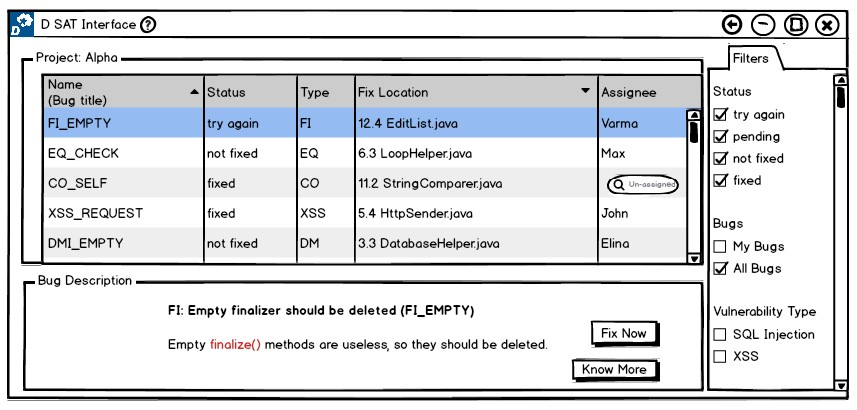
\includegraphics[width=\linewidth]{figures/d_tryagain}
	\caption{An interface prototype showing 'try again' status.}
	\label{fig:d_tryagain}
\end{figure}

Next, evaluate the designed prototypes as mentioned in \autoref{ch:researchmethodology_report}. After evaluation, requirements are gathered based on user feedback and also new findings from the literature, if any. New designs are prototyped as mentioned above and repeats as per User Experience Design cycle. \\ \\

\section{Research Question 3:  \\ How to Carry Traceability of Bug Fixing?}

\textbf{Solution ideas}: \\ \\
1. a timestamp for each bug fixing attempt with changes button \\
2. a Revert button \\ \\

With the above mentioned possible ideas, we design the prototypes. The prototype, i.e., Prototype 1 \ref{fig:d_changes} illustrates there is a timestamp for each bug fixing attempt which might help in the context of traceability as to know when someone is trying to mitigate a bug. Also, a button ‘Changes’ could perhaps show the code difference to the previous state of the codebase. The other prototype, i.e., Prototype 2 \ref{fig:d_revert}, illustrates in a situation where the user wants to revert to the previous situation of the codebase. This functionality could perhaps help in a situation when modified code introduces new bugs with an attempt to fix a particular bug. \\ \\

Next, evaluate the designed prototypes as mentioned in \autoref{ch:researchmethodology_report}. After evaluation, requirements are gathered based on user feedback and also new findings from the literature, if any. New designs are prototyped as mentioned above and repeats as per ‘User Experience Design cycle’. \\ \\

\textbf{Prototype 1}
\begin{figure}[hbt!]
	\centering
	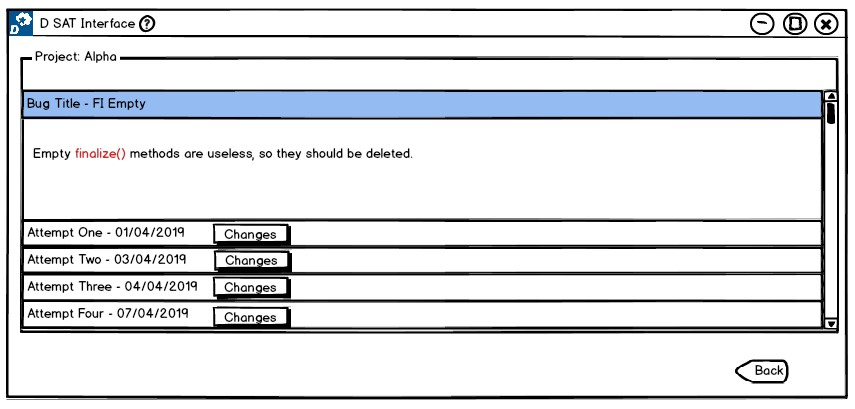
\includegraphics[width=\linewidth]{figures/d_changes}
	\caption{An interface prototype showing time stamp and changes button.}
	\label{fig:d_changes}
\end{figure}

\clearpage

\textbf{Prototype 2}
\begin{figure}[hbt!]
	\centering
	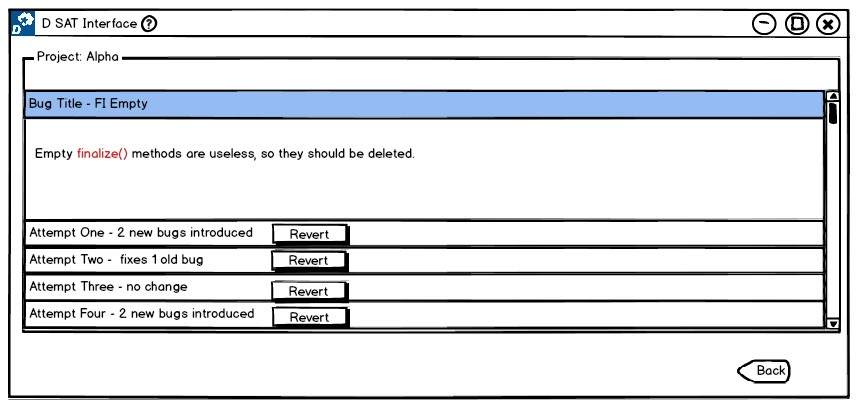
\includegraphics[width=\linewidth]{figures/d_revert}
	\caption{An interface prototype showing revert button.}
	\label{fig:d_revert}
\end{figure}

\let\cleardoublepage\clearpage


	